%%%%%%%%%%%%%%%%%%%%%%%%
%% Sample use of the infthesis class to prepare a thesis. This can be used as 
%% a template to produce your own thesis.
%%
%% The title, abstract and so on are taken from Martin Reddy's csthesis class
%% documentation.
%%
%% MEF, October 2002
%%%%%%%%%%%%%%%%%%%%%%%%

%%%%
%% Load the class. Put any options that you want here (see the documentation
%% for the list of options). The following are samples for each type of
%% thesis:
%%
%% Note: you can also specify any of the following options:
%%  logo: put a University of Edinburgh logo onto the title page
%%  frontabs: put the abstract onto the title page
%%  deptreport: produce a title page that fits into a Computer Science
%%      departmental cover [not sure if this actually works]
%%  singlespacing, fullspacing, doublespacing: choose line spacing
%%  oneside, twoside: specify a one-sided or two-sided thesis
%%  10pt, 11pt, 12pt: choose a font size
%%  centrechapter, leftchapter, rightchapter: alignment of chapter headings
%%  sansheadings, normalheadings: headings and captions in sans-serif
%%      (default) or in the same font as the rest of the thesis
%%  [no]listsintoc: put list of figures/tables in table of contents (default:
%%      not)
%%  romanprepages, plainprepages: number the preliminary pages with Roman
%%      numerals (default) or consecutively with the rest of the thesis
%%  parskip: don't indent paragraphs, put a blank line between instead
%%  abbrevs: define a list of useful abbreviations (see documentation)
%%  draft: produce a single-spaced, double-sided thesis with narrow margins
%%
%% For a PhD thesis -- you must also specify a research institute:
% \documentclass[phd,ilcc,twoside]{infthesis}

%% For an MPhil thesis -- also needs an institute
% \documentclass[mphil,ianc]{infthesis}

%% MSc by Research, which also needs an institute
% \documentclass[mscres,irr]{infthesis}

%% Taught MSc -- specify a particular degree instead. If none is specified,
%% "MSc in Informatics" is used.
% \documentclass[msc,cogsci]{infthesis}
% \documentclass[msc]{infthesis}  % for the MSc in Informatics
\documentclass[msc, deptreport,parskip]{infthesis}

%% Master of Informatics (5 year degree)
% \documentclass[minf]{infthesis}

%% Undergraduate project -- specify the degree course and project type
%% separately
% \documentclass[bsc]{infthesis}
% \course{Artificial Intelligence and Psychology}
% \project{Fourth Year Project Report}

%% Put any \usepackage commands you want to use right here; the following is 
%% an example:
\usepackage{amsmath, amssymb, amsfonts, amsthm, fouriernc, mathtools}
% My additions
\usepackage{algorithm}
\usepackage[noend]{algpseudocode}
%%%%%%%%%% CODE FORMAT  %%%%%%%%%%%%%%%%%%%
\usepackage{listings}
\usepackage{listings}
\usepackage{color}
\usepackage{pifont}
\usepackage{microtype} %improves the spacing between words and letters
\usepackage[colorinlistoftodos]{todonotes}
\usepackage{graphicx}
\graphicspath{ {./pics/} {./eps/}}
\usepackage{epsfig}
\usepackage{epstopdf}
\usepackage[bottom]{footmisc}
\usepackage{titlesec}
\usepackage{sectsty}
\usepackage{caption}
\usepackage{subcaption}
\usepackage[utf8]{inputenc}
\usepackage[english]{babel}
\usepackage{hyperref}
%% Information about the title, etc.
\title{Código Network: a Decentralized Firmware Update Framework for IoT Devices}
\author{Sotiris - Alexandros Nanopoulos}

%% If the year of submission is not the current year, uncomment this line and 
%% specify it here:
% \submityear{1785}

%% Optionally, specify the graduation month and year:
% \graduationdate{February 1786}

%% Specify the abstract here.
\abstract{%
With the number of Internet-of-Things devices increasing at an exponential rate, the need for secure and efficient firmware updates becomes a necessity. Additionally, the costs required to maintain the infrastructure that could serve firmware updates efficiently to large sets of users are a significant financial burden for small IoT device manufacturers. Furthermore, the current firmware update schemes do not allow open-source development, of firmware if the manufacturers decide to stop maintaining a device.

In the present work, we propose and implement a decentralized firmware update framework called Código network. For Código network, we set the following requirements: (i) no single point of failure, (ii) equivalent security with code signing, (iii) transparency of firmware updates and (iv) scalability. To fulfill the aforementioned requirements, Código network is implemented on top of the Ethereum blockchain and the IPFS network. In our developed system, developers upload firmware to a  repository, implemented as a Ethereum decentralized application. In parallel, users can browse the repository for trusted firmware and download the firmware. To encapsulate trust in a decentralized network, we develop an open-source implementation of Web-of-Trust as an Ethereum smart-contract. 

The performance of Código network is quantified based on two criteria. The first criterion is the transaction costs entailed in the operation of the Ethereum smart contracts. The second criterion is the time required to distribute a new firmware to a set of users. To evaluate it we compared Código network with the Client-Server model and BitTorrent. The simulation tool we developed is under code review in order to be added in the IPFS test framework.
}
%% Now we start with the actual document.
\begin{document}

%% First, the preliminary pages
\begin{preliminary}

%% This creates the title page
\maketitle



%% Finally, a dedication (this is optional -- uncomment the following line if
%% you want one).
% \dedication{To my mummy.}

%% Create the table of contents
\tableofcontents

%% If you want a list of figures or tables, uncomment the appropriate line(s)
% \listoffigures
% \listoftables

\end{preliminary}

%%%%%%%%
%% Include your chapter files here. See the sample chapter file for the basic
%% format.

%% Sample chapter file, for use in a thesis.
%% Don't forget to put the \chapter{...} header onto each file.

\chapter{Introduction}{

\section{The Internet of Things Era}{

The past decades were the decades when the World-Wide-Web penetrated our life. As the time passes and technology advances, humans find more clever ways to integrate Internet technology to improve our lives, become more efficient and tackle problems that previously seemed impossible. Robotics, virtual reality, the Internet of Things, the cloud and artificial intelligence move from the pages of science-fiction books to the reality. Utilizing these novel technologies is expected to make a new industrial revolution and reshape the industry entirely. For that reason, governments around the globe form their strategic plan around arising technology. The German government has already published their high-tech policy that aims to reform their industry, called \textit{Industry 4.0} \cite{lasi2014industry}. Meanwhile, the Chinese government is pushing an initiative to comprehensively upgrade their industry, \textit{Made in China 2025} \cite{kennedy2015made}, which is based on the applications of new technology to reform the manufacturing and supply chain industries.

A core part of this technological revolution is the Internet of Things (IoT). IoT can be defined as a set of connected devices that are capable of communicating with the rest of world in the form of sending and receiving data via the Internet \cite{said2013towards}. IoT shines in industrial applications, as it provides a mean of communication between machines and computers. This communication could be used to collect data during operation and to proactively take action based on the data. However, IoT applications are not limited to the industrial environment. Smart-homes, fitness trackers and autonomous cars are domains in which IoT has its rightful place. With all those applications of IoT devices we expect a dramatic increase in its adoption rate. In particular, ARM predicts the number of use cases of IoT will increase and exponentially and that 1 trillion IoT devices will be deployed by 2020 \cite{Sparks2017TheDevices}. The exponential increase int the number of IoT devices creates the need for efficiency in every aspect of an IoT device. The devices need to collect data, process data, communicate with the Internet and update their firmware efficiently.
}

\section{Firmware Distribution}{

Updates are a crucial part in the lifetime of any software. Software updates are the only reliable way to make a software stand against the test of time. Software updates add features, improve the efficiency and remove bugs from the software. Besides performance, software updates also fix security vulnerabilities, improve the security of the system and address known and potential attacks against the software. Consequently, it would be wishful thinking to imagine a software that does not need any update in its lifetime. However, especially in the case of IoT devices and firmware updates, updating is are one of the most vulnerable phases in the lifetime of the device \cite{Shamir2017SummaryCryptography}. The reason for that, is the high computational cost entailed in applying cryptographic primitives. As a result, many manufacturers tend to either not use them at all or use insecure implementations.

Firmware distribution is a specific type of content distribution that aims at delivering a single firmware file with a size of ~5-15 MBytes from a firmware developer to an end device. Traditionally the architecture of firmware updates for IoT devices is the one illustrated in Figure \ref{fig:FirmUpd}. The IoT gateway (i.e. a personal computer or a smartphone) will download the firmware from the manufacturer server. Then the gateway will verify the origin of the firmware based on a specified code signing protocol and push the firmware to the end-device using a Wireless Local Area Network (WLAN) protocol such as Bluetooth \cite{fitbit}.

\begin{figure}[htb!]
\centering
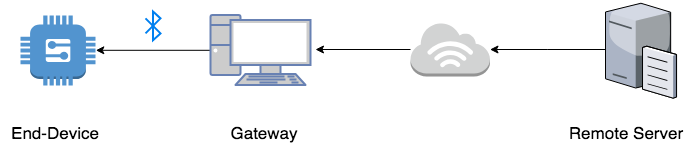
\includegraphics[width=0.95\textwidth]{./pics/Firmware_updates.png}
\caption{Traditional IoT architecture for distributing firmware updates}
\label{fig:FirmUpd}
\end{figure}

Firmware updating, is such a sensitive process that it spawned a new attack surface against embedded devices called firmware-modification attacks \cite{7804660}. Firmware modification attacks can have devastating effects on the device. Modified firmware can transform the device into a spyware and steal sensitive information from the user. They can disable the device bootloader, thus making it extremely hard to update the firmware of the device and remove the malicious firmware. In general, once a malicious firmware is injected, the device becomes the hostage of the attacker. Interested readers can refer to the paper of Classen et. al. that illustrates different attacks that rely on the firmware-modification attack \cite{Classen2018AnatomyFirmware}.
}

\section{Problem Definition} \label{sec:PD}{

In this project we aim to develop a decentralized firmware update network that would enable open-source development of IoT firmware. Open-source development of firmware benefits are twofold. Firstly, it enables patching vulnerable firmware even if the device manufacturer goes bankrupt. Secondly, open-source development enables transparency and code review. The user can review the code to know exactly what data are gathered from her and how they are being used. This transparency is crucial given the nature of IoT applications in home automation and wearable devices.

For our decentralized firmware update network we set the following requirements:
\begin{itemize}
    \item \textbf{No single point of failure}: The users should be able to retrieve a new firmware even in the case that a single node fails. Making the system resistant to single point of failures will also implicitly allow open-source development of firmware. Device manufacturers may have an advantage over others, however this advantage should not prohibit developers from developing new firmware for a device. 
    \item \textbf{Equivalent security with code signing}: The system should not make any security discounts over the current status quo, which is code signing.
    \item \textbf{Transparency}: Firmware updates should be eponymous, immutable and persistent. Any user should be able to retrieve and browse through the firmware releases for a given device.
    \item \textbf{Scalability}: The firmware release should be distributed and evenly balanced. Nodes participating in the network should contribute by uploading firmware they have to other peers and be able to download firmware they want from peers.
\end{itemize}

}

\section{Our Contribution}{

The goal of this project is to design a decentralized firmware update framework for IoT devices. To that end, we contributed in the following ways:

\begin{enumerate}
    \item We developed a smart-contract that models trust in decentralized environments. The implementation was based on the idea of Web-of-Trust. To our knowledge there is no publicly available implementation of Web-of-Trust in an Ethereum smart-contract.
    \item We developed a smart-contract that performs the business logic of a firmware repository. The firmware repository is feeless for the users and the fees required by the developers are minimal.
    \item We designed and developed the Código network clients that meet the requirements set in Section \ref{sec:PD}. Código network interacts with the Ethereum and IPFS networks in a user-friendly way. We measured the costs entailed in using the Código network.
    \item We designed a simulation tool to measure the performance of IPFS and used this simulation tool to compare the performance of IPFS against the Client-Server model and BitTorrent.
    \item The  features we added to the IPFS simulation framework and the performance results received attention from the IPFS community \footnote{\url{https://github.com/ipfs/go-ipfs/issues/5226}} and spawned a fruitful discussion on the current implementation. Our findings point to the main performance issues of IPFS. Additionally, we made the first comparison between IPFS and BitTorrent. The developed code is now under code-review in order to be included in the IPFS testing framework.
\end{enumerate}

}

\section{Project Outline}{

The rest of this project is organized as follows: Chapter \ref{chap:bc} aims to provide the reader with sufficient background information on Blockchain technology and Ethereum decentralized applications, in order to understand the evaluation of Código network smart-contracts.  Chapter \ref{chap:cn} presents and compares the most common approaches used for file distribution. Chapter \ref{chap:CNDesign} documents our design of Código network. In this part, we focus on modeling trust and implementing the smart-contracts and the UI clients developed. Additionally, the performance of the developed Ethereum smart-contracts, measured in terms of transaction costs, is presented. For completeness we evaluate closely related work. In Chapter \ref{chap:CNeval} a comparison between different file distribution frameworks is presented. Additionally, the experiment setting and the simulation frameworks developed and used to perform the comparisons are presented. In chapter \ref{chap:conc}, an overall analysis of completion of the project is presented. The assessment is based on the requirements set in Section \ref{sec:PD} and some ethical consideration that arose during the project are presented. Finally, the project is concluded with proposals for further research.

}

}


\chapter{Blockchain Technology} \label{chap:bc}{

The blockchain revolution began with the Bitcoin whitepaper \cite{nakamoto2008bitcoin} that demonstrated a protocol for maintaining a log of transactions in trustless settings in which peers can enter and leave the protocol execution at any point. The Bitcoin whitepaper uses this protocol to create the first decentralized digital currency (cryptocurrency). In this section, a brief introduction to the blockchain technology will be presented. Finally, the Ethereum blockchain \cite{WoodGavin2014Ethereum:Ledger}, which is used as a building block for Código network, will be examined in more detail.

\section{Maintaining a Chain of Blocks}{

\subsection{Transactions}{
The blockchain technology consists of a set of protocols and algorithms that enable a set of trustless peers to maintain, extend and agree on a common distributed log of ordered transactions. The underlying distributed log of ordered transactions is implemented using the blockchain data structure in the majority of cases. The blockchain is a recursive data structure similar to a linked-list. Each block in the blockchain contains a cryptographic pointer to the previous block. The existence of cryptographic pointers connecting the blocks gives this data-structure a particular set of properties. That if one block within the chain changes, then the whole chain after that also needs to be recreated to make the pointers match. Then, assuming that the process of creating valid blocks is "hard", the distributed ledger has one really useful property which is tamper resistance.

According to the Bitcoin protocol (this also holds true for all blockchain protocols), each node of the system needs to have its own copy of the blockchain. The blockchain of the user is synchronized with other blockchains using the respective blockchain client. Similarly to most distributed systems applications reading the blockchain is a straightforward procedure. The users parse their own local blockchain and perform the calculations they wish. On the other hand, writing data to the blockchain entails a more complex procedure. In order to write to the blockchain, the user needs to perform a transaction. Different blockchains will have different transaction types. For example, in Bitcoin sending 1 BTC from Alice to Bob would require a transaction, whereas in Ethereum changing the value of a smart-contract variable from 0 to 1 would require a transaction.

Users who want to make a transaction will have to make the following steps to write it in the blockchain. Create a valid transaction according to the blockchain protocol, select the transaction fees, sign the transaction and then broadcast it to the network. A miner will select a number of transactions that float in the network and organize them in a block. Then the miner will try to append that block to the blockchain. The rules for appending blocks to the blockchain are described in the consensus protocol of the blockchain. The consensus protocol is a crucial component of each blockchain and it is the component that guarantees that all participants of the network will eventually agree upon a unique transaction log. In Section \ref{sec::BcCons} the consensus layer will be examined in more depth.

Transaction fees and transaction order are subtle topics especially when building applications on top of blockchains. Blockchain technology offers no guarantee about the absolute order of transactions. This means that Alice could send a transaction minutes (even hours) later than Bob and still see her transaction first on the blockchain. Most miners, assuming a rational behavior, will choose to add a transaction with high transaction fees to the blockchain. This asynchronism in the transactions leaves a lot of room for attacks when designing an application. Blockchain applications should be designed in a way that ensures fairness for the users. This means that users should have the same experience when using the application, regardless of the transaction order \cite{Luu:2016:MSC:2976749.2978309}.
}
\subsection{Consensus} \label{sec::BcCons}{

The consensus protocol used by the Bitcoin and the Ethereum blockchain relies on Proof-of-Work (PoW). According to the protocol, in order to produce a new block, miners need to solve a moderately hard cryptographic puzzle. The cryptographic puzzle required is finding a nonce such that the hash of the previous block concatenated with the nonce is less than a target difficulty \cite{nakamoto2008bitcoin}.

The goal of any blockchain protocol is to maintain a robust transaction ledger. The robust transaction ledger can also be thought of as a state-machine-replication protocol (this is more aligned with the distributed systems literature). A transaction ledger is said to be robust if it satisfies two properties: persistence, and liveness. Intuitively, the persistence property guarantees that when transactions are added to the blockchain they cannot be edited and all honest parties agree upon their position in the blockchain. The liveness property guarantees that all valid transactions will be eventually added to the blockchain. For a more rigorous definition of these properties, the reader can refer to \cite{Garay2017The,Pass2017AnalysisNetworks,Kiayias2016OnBlockchain}. The above papers proved that the Bitcoin and the Ethereum consensus protocols generate a robust transaction ledger under the assumption that more than 50\% of the hashing power of the network belongs to honest parties. To construct those proofs, these papers also make assumption on network delay. However, rigorously evaluating these papers is out of the scope of the project. 
}

\subsection{Blockchain Zoo}\label{sec:blockchainZoo}{

A lot of the details in the description above are left obscure by choice. The reason for that is because the design of a blockchain entails many subtle choices. Many research papers have tried to organize different blockchains based on their design choices \cite{Vukolic2016TheReplication}. There are blockchains that focus on maintaining a robust transaction ledger of a cryptocurrency, such as Bitcoin or Litecoin. There are blockchains that focus on state machine replication such as Ethereum where a user can provide the blockchain with an arbitrary state and other users can modify the state using functions. There are blockchains where nodes can enter or leave the protocol execution at any time. These blockchains are called public. Contrary there exist blockchains where only a limited number of users can participate and/or there are restrictions on who can issue new transactions and/or produce blocks. These blockchains are called private.

Designing a blockchain application requires to select the proper blockchain for your problem or creating a new blockchain from scratch. Creating a new blockchain application from scratch is no an easy task. It requires to carefully design all the details, implement them correctly and have a sufficient amount of users to make the network secure. On the other hand, piggybacking on a pre-existing blockchain creates limitations, as the designer will have to fit the application requirements in the existing infrastructure.
}
}
\section{Ethereum Blockchain}{

\subsection{Smart-Contract Programming}{

In general, a contract is a binding agreement between parties that clearly define the responsibilities and duties of the stakeholders. Contracts are used widely in the world to construct and formalize business and other agreements between people. In his paper, Szabo \cite{szabo1997formalizing} proposed the idea of digital contracts that would be developed by the stakeholders in the form of programs and then executed by machines. An example of such digital contract is the firmware of a vending machine. It is programmed by the stakeholders to provide the user with a refreshment drink upon the insertion of a coin.

Quickly after the Bitcoin revolution, people understood that the Bitcoin scripting language offered an infrastructure to develop and deploy smart-contracts. The Bitcoin scripting language offers many possibilities to develop smart-contracts that implement $m-n$ multi-signature transactions, coinjoin \footnote{\url{https://en.bitcoin.it/wiki/CoinJoin}, Access Date: 7 Aug. 2018} transactions or even hosting a domain-name-system \cite{kalodner2015empirical}. However, the Bitcoin scripting language is limited by design to a specific set of instructions and does not offer functionalities such as loops. This causes the Bitcoin scripting language to not be Turing-Complete. This design choice by Bitcoin led to the development of Ethereum. Ethereum was designed to be a fully programmable blockchain which supports a Turing-complete language. This means that, in theory, any computational problem could be solved in Ethereum. 

Ethereum smart-contracts are developed in a higher level language such as Solidity and then compiled down to native Ethereum-Virtual-Machine (EVM) instructions. With this design, Ethereum managed to create an entire ecosystem of decentralized applications (DApps). Ethereum applications can have a smart-contract to play the role of a decentralized server that is fully determined by code. However, this comes at a significant cost. Decentralized applications are not private, they operate on public data in a fully transparent way.
}
\subsection{Ethereum Smart-Contract Implementation}{

Contrary to Bitcoin, Ethereum follows more strictly the state-machine replication definition in its blockchain design \cite{WoodGavin2014Ethereum:Ledger}. The Ethereum network can natively handle monetary transactions using its own currency called ETH but is not limited to that. Users can define arbitrary states and state modification functions on the blockchain. The states are implemented as smart-contracts, which are files of code that resemble, at least syntactically, to classes. The smart-contracts contain variables (state variables) and functions that provide an interface to modify the state. As a result, in the Ethereum network, a transaction can have the following form. Alice wants to execute function \textit{foo} from smart-contract \textit{bar}. Then the miner would execute the function in the smart-contract locally on his computer, update the state, add the transaction to the blockchain and return the results to Alice.

Now consider a malicious function in a smart-contract that is an infinite loop. Eve could send a transaction with a request for executing this malicious function. The miner who sees the transaction and tries to execute the function is suffering from a denial of service attack. The miner is trying to execute a program that never ends and cannot continue the mining operation. To prevent this attack, Ethereum uses the notion of a unitless quantity called \textbf{gas}. Each EVM instruction is associated with a \textbf{gas cost}. The issuer of an Ethereum transaction needs to specify the following, (i) the gas price which has monetary value and (ii) the gas limit. As a result, an Ethereum transaction will have transaction fees that can be calculated in the following way:

\begin{align*}
 (transaction\_fees) = (gas\_cost) \cdot (gas\_price)
\end{align*}

and the gas cost is calculated in the following way:

\begin{align*}
 (gas\_cost) = min\{(gas\_limit),(inscruction\_costs)\}
\end{align*}

If the gas cost of the instructions surpasses the gas limit set by the user the execution of the function is stopped and the state of the smart-contract is reverted. For the transactions, miners are rewarded with fixed block reward and with the transaction fees required to execute smart-contract functions, for appending a new block to the blockchain. As a result, setting a high gas price for your transaction would incentivize miners to add it in the next block.

Storing data on the blockchain also comes with a cost. This is another benefit of the gas cost, that it incentivizes users to store the minimum amount of information in the blockchain. As a consequence of that, instructions (OPCODEs) that reduce the data that need to be stored on the blockchain have a negative gas cost. For example, the delete OPCODE used to delete an entry from an array is associated with negative gas cost. Note that, even though there exist operators with negative costs, it is impossible to create a negative gas cost transaction, as it is not possible to create a function that only uses a delete OPCODE.
}
}
}

\chapter{Content Delivery} \label{chap:cn}{

The content delivery problem can be defined as the problem of efficiently distributing a file from an origin, possibly the creator, to a set of user. This problem arises every time a user tries to view a website, requests the delivery of an HTML file, watches a video on YouTube, requests the delivery of a video file and updates the Operating System (OS) of her computer, or requests a new ISO version of the OS. To address this problem, multiple approaches with different performance guarantees are employed. In this section, the most common content distribution methods will be discussed and compared.

\section{Client Server Model}{

The first approach to address content delivery is the client-server model. The client-server model relies on the existence of one or multiple servers operated by the file distributor \cite{Berson:245910}. Clients that want the file make a request to download it from the server and then the server responds back with the file. This paradigm is widely used to deliver the front-end of a website to the user. When a user visits a website such as google.com, the browser requests the HTML file from a Google server. This approach works perfectly for small HTML files. Companies can use cloud-services to vertically and horizontally scale their infrastructure to handle an increasing number of requests. However, as the file sizes and the number of requests increase, the scaling required eventually becomes prohibitively expensive. As a result, the website becomes slow and ultimately unavailable. The other disadvantage of this approach is that it relies on a single entity to distribute the file. If this entity becomes unavailable, chooses to censor a file or the government bans the access to the distributor then the file becomes unavailable.
}
\section{End-host Multicast}{

End-host multicast is an improvement over the client-server model that focuses on improving its performance in distributing larger files to multiple peers. There exist two versions of multicast. IP multicast relies on the idea that routers forward packets to multiple addresses. End-host multicast relies on the idea that each end-host sends the downloaded files to others when it finish downloading. Unfortunately, IP multicast, although technologically viable, is not widely supported by Internet-Service-Providers and as a result, it is a viable solution only for distributing content within a private network (e.g. a data center). End-host multicast relies on the idea that when nodes successfully finish downloading a file, they themselves distribute the file to two other nodes. The benefit of this approach is that it moves some of the load from the distribution server to end-hosts. Various protocols such as Overcast \cite{jannotti2000overcast} and ALMI \cite{verma2001almi} have been designed in the past decades. All the designed protocols create a single tree structure as illustrate in Figure \ref{fig:ipMulti} to distribute the file.

\begin{figure}[htb!]
\centering
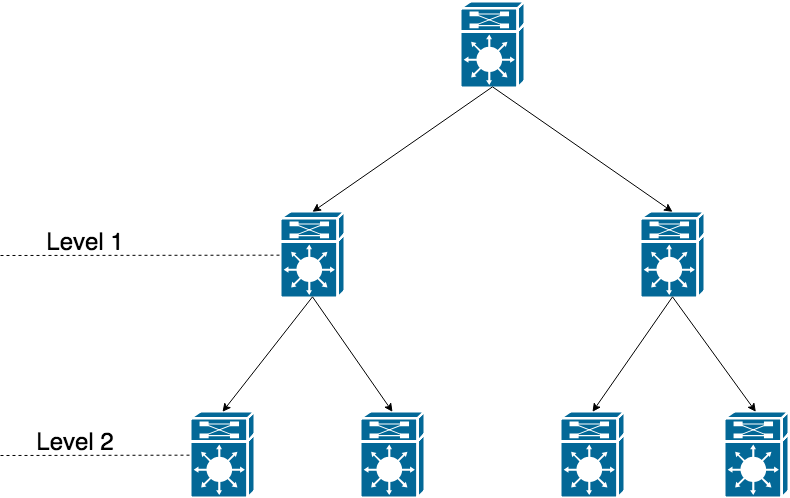
\includegraphics[width=0.95\textwidth]{./pics/Ip-multi.png}
\caption{End-host multicast single tree structure and propagation of data}
\label{fig:ipMulti}
\end{figure}

The main issue with the single tree structure is poor load balancing among nodes. The first observation is that nodes in the lowest level do not contribute at all to the distribution of the file. Additionally, if a node at a high level, close to level 0, fails to distribute the file or is terribly slow, then the whole subtree that depends on it will not receive the file.

}
\section{BitTorrent}{

BitTorrent is a peer-to-peer (P2P) file distribution protocol that was designed by Brah Cohen in 2001 \cite{BramCohen2008BitTorrentSpecification}. BitTorrent was a more decentralized version of previous systems such as Napster and Kazaa. According to the BitTorrent protocol nodes that are interested in downloading the same file are organized in swarms. Within the swarm, nodes request chunks of the file from their neighbors.

A really innovative idea in the design of the BitTorrent protocol is the "tit-for-tat" mechanism. This mechanism incentivizes nodes to contribute to the distribution of the files because otherwise they will be choked by their neighbors. This means that in order to download all the chunks of the file, one must also upload chunks of they file you already have.

To distribute a file using the BitTorrent protocol, the creator must create a torrent file that specifies the address of the swarm-tracker, the chunks that compose the file and their hash. The torrent file is uploaded in a torrent repository and then users can download the torrent file and feed it to a BitTorrent client. Finally, the BitTorrent client will download the original file. In terms of performance and robustness, BitTorrent has already proved itself  \cite{BitPerf}. According to the study in \cite{6912519}, P2P content distribution constitutes 16\% of the download traffic of two major European ISPs. Furthermore, companies like Facebook, Twitter, Blizzard \footnote{\url{http://us.blizzard.com/es-mx/company/about/legal-faq.html}, Access Date: 7 Aug. 2018}, and Linux foundation \footnote{\url{https://linuxtracker.org/}, Access Date: 7 Aug. 2018} use their in-house implementation of the BitTorrent protocol to distribute data among data centers or to their users.

The main robustness drawback of the BitTorrent protocol is that it has single-point of failure. If the swarm-tracker becomes unavailable (due to censorship), then users have no mean to enter the swarm and download the file. In terms of performance, the main issue with BitTorrent is data duplication. This means that if the same file is uploaded with a different name, then there will be two torrent swarms that do not communicate with one another.
}
\section{IPFS}{
IPFS\footnote{Interplanetary File System} is also a peer-to-peer (P2P) file distribution protocol that was designed by the Protocol Labs company and 
Juan Benet in 2014 \cite{benet2014ipfs}. Protocol Labs received 257M in funding in 2017, that was the biggest Initial Coin Offering (ICO) at the time \footnote{\url{https://coinlist.co/filecoin}, Access Date: 7 Aug. 2018}. IPFS is a decentralized file distribution protocol that shares many ideas with BitTorrent but uses the hash of the file as its address in the network. IPFS can be thought of as a single swarm BitTorrent network. Similarly to BitTorrent, IPFS uses the "tit-for-tat" mechanism to incentivize users to distribute their files. However, as users are organized in a single swarm, a user can distribute chunks of a different file than the ones she tries to download.

Users entering the IPFS network download a ledger that contains a list of nodes that participate in the network. Then the node can make a connection to the users she sees in the ledger. Upon establishing a connection to the network, the user can locate other nodes that have the files she wants and download the files from them. In return, she uploads the files she already has. This is implemented with two lists. Each user publishes to the network her want list, i.e. list of file chunks that she wants, and the have list, i.e. a list of file chucks that she has.

As an optimization to avoid storing duplicate data in the network, files are stored based on their hash, thus constructing a Merkle Tree \cite{MerkleTrees} with different files and versions of files. Each file is identified with an IPFS link that has the following form:
\begin{center}
/ipfs/\textit{file\_hash}/
\end{center}
IPFS links are resolved using the IntePlanetary-Name-System (IPNS) which is similar to Domain-Name-System (DNS) but for IPFS links. As an example, a website could be hosted on IPFS using the following link:

\begin{center}
localhost:8080/ipfs/\textit{hash(my\_website.html)} 
\end{center}


The main disadvantage of IPFS at the time of writing is the exponential increase of available files. Take for example the HTML page for the landing page of a website. Small differences in HTML would result in a completely different hash. As a result, IPNS that resolves the name of the website to an IPFS address must constantly be updated, even for small changes of files. Another performance issue arises from the immaturity of the project. As the project is in an early Alpha development stage many operations are not optimized. As we will later demonstrate, this suboptimal operations severely limit its practical performance.
}

\section{Summary}{

A comparison between the content distribution protocols discussed in this section is presented in Table \ref{tab:CNComp}. The comparison focuses on the scalability of the protocols as the number of nodes increases, the existence of failure points within the network and how balanced the load is among the participants in the network.

\begin {table}[htb!]
\caption {Comparison of content distribution protocols} \label{tab:CNComp} 
\begin{center}
 \begin{tabular}{|c| c|c| c|c| c|c| c|} 
 \hline
  Protocol & Scalability & Point of failure & Load Balance \\ [0.5ex] 
 \hline
 Client-server & Depends on server & Server & Poor  \\ 
 \hline
 End-host multicast  & Depends on each node & Multiple partial & Poor \\
 \hline
 BitTorrent  & No scalability issues & Tracker server & Evenly Distributed \\
 \hline
 IPFS  & No scalability issues & None & Evenly Distributed \\
 \hline
\end{tabular}
\end{center}
\end {table}

}

}

\chapter{Código Network Design}\label{chap:CNDesign}{

In this project we propose, design and implement, Código network \footnote{\url{https://github.com/davinci26/Codigo-Network}}, a decentralized firmware distribution system for IoT firmware. At its core it relies on Blockchain technology and IPFS. To achieve such design, the first step is to construct a thread model and make valid security assumptions. Another recurring issue in decentralized systems that rely on user created content is trust modeling. Código network uses its own implementation of Web-of-Trust to provide users a mean of selecting which firmware to download for their IoT device. Finally, in this section the Código network and its components, Ethereum smart-contracts and clients, are thoroughly presented.

\section{Closely Related Work}{

The intersection of IoT and blockchain has received a lot of academic and industrial attention over the past few years \cite{Christidis2016BlockchainsThings}. The majority of applications that integrate blockchain technology in the IoT ecosystem propose the replacement of cloud persistence storage such as SQL and NoSQL databases, with a distributed ledger \cite{HUCKLE2016461}. The main advantage of this replacement is that multiple parties could simultaneously read and write in the ledger in a secure and transparent way. This leads to less business-to-business communication overhead and theoretically improves the current status quo \cite{KouzIoTBC}. A prime example of this approach is the integration of IoT and blockchain to simplify the supply chain industry with blockchain applications such as IOTA \footnote{IOTA: \url{https://www.iota.org/, Access Date: 7 Aug. 2018}} and VeChain \footnote{VeChain: \url{https://www.vechain.org/}, Access Date: 7 Aug. 2018}.

Another point of intersection of IoT and blockchain is secure distribution of firmware updates. This intersection point is new and is only explored by a few research papers. One particular research paper explores the idea of designing a new blockchain to distribute firmware updates \cite{Lee2017Blockchain}. The main benefit of their approach is that devices would be able to check the blockchain to see if a new firmware has been pushed by the manufacturer. The main drawback of their approach is that, even with a blockchain, their system is still centralized towards the firmware manufacturer. Additionally, as their work relies on a new blockchain, the amount of engineering work, as discussed in Section \ref{sec:blockchainZoo}, required to transform this from a theoretical concept to a proof-of-concept is substantial.

Another research paper that tries to integrate blockchain technology to IoT proposes a low consistency blockchain that is suitable for the IoT ecosystem \cite{Dorri2017TowardsIoT}. The motivation behind their approach is to eliminate the PoW component of the blockchain. The question that arises in their design is how consistency is ensured if no consensus algorithm is provided. In their paper they propose a way to do so but they do not provide rigorous mathematic arguments on the security of their approach. Based on their network they also built a firmware distribution scheme 
\cite{Steger2017SecureConcept}. Their scheme is also centralized and heavily relies on the manufacturer to produce new firmware updates.

The last research paper that is closely related to the scope of the thesis is the CHAINIAC project \cite{nikitin2017chainiac}. In their paper they present a novel system that utilizes an authenticated data structure (Skipchains) and verified builds to achieve secure software updates. Their system is decentralized and does not contain a single point of failure. The interesting idea in their project is that developers instead of signing the binary file they sign the source code. The source code is signed by $m-n$ developers. The use of a multi-signature scheme makes the system resistant to compromised signing keys. Then an intermediate pool of verifiers is responsible for building the software (verifiable builds) and endorsing it. The endorsements are stored in a data-structure similar to blockchain called skipchain. The only weak point in their design is the lack of incentives for the verifiers. Verifiers do not receive any reward for spending computation resources on building large software projects and thus have weak incentives for providing this service. This weakness only affects the system in case of real-world deployment.
}

\section{Threat model and Security Assumptions}{

A crucial part in the design of a secure decentralized application, is the identification of possible adversaries, their incentives and their power. Código Network has many similarities with the OpenBazaar e-commerce platform \footnote{OpenBazaar is decentralized marketplace similar to Ebay, that uses blockchain and cryptocurrencies to perform transactions.}. The main difference of the two is that Código has a more narrow focus on peer-to-peer (P2P) distribution of firmware for embedded devices. The combination of the Código's narrow focus to IoT firmware and the lack of monetary transactions makes it less vulnerable to attacks. This is is due to the fact that nodes that only use the system to receive firmware updates have no immediate incentives to deviate from a proper execution of the protocol (This does not apply to OpenBazaar). Only users that develop firmware have incentives to attack it. As a result, the system should be designed to protect users from malicious developers that want to infect embedded devices with malicious software.

A malicious developer is an agent in the network that will upload a "firmware" to the network knowing that the firmware is either not working or is exploitable in some way. The benefit of polluting the network with unusable software is to grief other users of the system and cause denial of service. Polluting the network with exploitable firmware comes with many financial advantages \cite{Classen2018AnatomyFirmware}. A subtle observation is that in both cases the reward to the malicious agent is either non-monetary or even if it is monetary, then the reward comes from a source outside of the network. As a result, it is not possible to model the firmware developers as rational agents and use a game-theoretic approach to enforce them to follow the protocol. Another subtle observation, is that the adversary is in a favorable position in decentralized environments compared to centralized ones. In the decentralized setting the attacker can generate multiple identities and use them  to attack the system. Essentially, in any decentralized system it is impossible for a user to determine if she is interacting with one or multiple users. Additionally, the pseudo-anonymity that comes in every decentralized application makes it harder for users to trust other agents of the network.


To protect Código Network from the aforementioned adversaries we assume that the following hold true:
\begin{enumerate}
\item Cryptographic primitives such as digital signatures, RSA public key encryption, AES encryption with padding are secure and there is no efficient algorithm that produces collisions on the hash functions SHA-256, SHA-3.
\item The frameworks used (IPFS, Ethereum) are theoretically secure and implemented correctly.
\item The programming languages used and the libraries used to develop the system are secure. Namely Python 3 programming language, web3-py, pyipfs and Py-Qt5.
\item \label{ref:curation} Nodes downloading a firmware are able to detect malicious firmware using hardware virtualization tools \cite{SpinkThomas2017Echv} or malware classfication software \cite{aspinall}.
\item The embedded device used are secure, unless already compromised.
\item The user is responsible for the security of her private keys. This is a common practice in the cryptocurrency ecosystem that is summarized by the following quote: "Not your key? Not your Bitcoins"\footnote{\url{https://tinyurl.com/ybdf6ffw}, Access Date: 7 Aug. 2018}.
\end{enumerate}

An important observation should be made on the \ref{ref:curation}th security assumption. This assumption is both theoretically reasonable and solves an important issue for Código network. Although \cite{aspinall} is limited to classifying android malware, the fact that their methodology focuses on Semantic-Based-Features means that it could potentially be modified and used to classify arbitrary firmware. This simulation to generate Semantic-Based-Features could be in sandbox environment that emulates the underlying embedded device hardware. In particular, with this assumption the system is able to address the content curation issue that arises in decentralized systems. With this assumption, it follows that nodes are able to distinguish on their own whether a firmware is malicious or honest, after downloading it.

}

\section{Modeling Trust in Decentralized Environments}{

Trust in decentralized networks is an open research area that lays outside the primary scope of this project. However, as it plays a crucial role in the system, it would be a big omission not to address it, even partially. To do so, various solutions that are widely used in practice and have some theoretical background have been considered. Before delving into the available solutions, the trust-sensitive operations of Código Network must be identified.

A requirement specific to Código Network is that, naturally, the manufacturer of the IoT system is a trusted party. As a result, as long as the manufacturer is actively maintaining the system, there exists a firmware that is infinitely trusted by nodes. Nodes are still free to choose any firmware they want, but they acknowledge the risk involved in their decision. When the manufacturer stops maintaining the firmware, the firmware owners will be incentivized to seek alternative firmware developed by the community. This is the point when nodes lose their infinitely trusted firmware and need to shift their trust to an unknown developer.

A naive solution to the problem is to use a star based rating system for each developer. This solution is inadequate as a malicious developer could easily create multiple accounts (Sybil Attack) and rate himself with the highest rating, thus making the rating system useless. Various heuristics, such as not counting the votes of new users, could be employed to alleviate Sybil Attacks. Such heuristics are easy to deploy but hard if possible at all to optimize with respect to the user experience. For this reason, we chose to avoid such design for a more robust solution.

In general, people tend to trust less people who are not committed in their actions. This is the problem a traveling saleswoman faces in her quest to sell her merchandise. The customers trust her less, because if she sells them a bad quality product then she has practically nothing to lose. A common workaround to this problem is providing the system with a form of commitment (Note that commitment here does not mean cryptographic commitment). In the real world the commitment comes from opening a store. In the digital world commitments can come in numerous ways, such as providing the system with valid computational PoW or by burning/donating some wealth. This kind of system, is also used in Código Network with dual benefit. Firstly, it increases the trust of users in the developers and also increases the cost of Sybil Attacks. Additionally, to make the system more resistant to Denial-of-Service attacks, the cost of uploading a new firmware exponentially increases for uploading new firmware within the same day. The uploading cost is either payed in terms of electricity, in case of PoW, or in terms of cryptocurrency, in case of Proof of Donation/Burn.

From the literature the following approaches were identified for addressing trust issues in decentralized systems.
\begin{enumerate}
\item \textbf{Web-of-Trust}: The Web-of-Trust is an old idea that is currently used in the PGP project \cite{ZimmermannPGP}. Intuitively, it is a mechanism to generate a graph with vertices representing users and edges representing the existence of trust between users. Then trust is quantified as the number of edges required to reach from one user to an other. With this approach trust is relative. In the Código Network setting this means that different users will trust different firmware. As a result, trust should be calculated every time a node queries the smart-contract.

\item \textbf{Stake as trust}: Stake as trust is a novel idea that on an intuitive level shares some commonalities with the Proof of Stake concept. This idea emerged from discussions during the project. The idea is based on the fact that a user who allocates a lot of stake as an initial investment to upload her firmware into the network is incentivized to have developed a trustworthy firmware. An advantage of this approach is that the trust users allocate to a firmware is uniquely defined for all users.

\item \textbf{Trust-is-Risk} \cite{cryptoeprint:2017:156}: The basis of these modeling is to quantify trust with a monetary value. This idea is particularly useful in the context of decentralized marketplace in which users perform financial transactions to buy goods from other users. According to their paper, user Alice should she trust Bob, she will deposit $X$ BTC (or any other cryptocurrency) into a shared wallet. Assuming that this kind of wallets of are widely used within the network then if Alice wants to buy a service from a Charlie then she can use a chain transaction between all the shared wallets. Then if the service that she is buying costs less than then her initial deposit of $X$ BTC, she is not taking any more risk.
\end{enumerate}

From an academic perspective both stake as trust and Trust-is-Risk have a solid mathematical background. However, neither is robustly implemented and deployed into a real world application. Additionally Trust-is-Risk is particularly useful when users perform financial transactions. This is not the case in Código network. For this project, Web-of-Trust is chosen to model trust. The reasoning behind this choice is the successful deployment of Web-of-Trust in PGP and OpenBazzar.

Web-of-Trust gives Código network an additional security property, Sybil attack resistance. The influence of a developer in the network and the visibility she gets depends on other people trusts. As a result, creating new accounts that do not belong in the trust graph does not come with an advantage. New accounts are disconnected (isolated) vertices in the trust graph.

}
\section{Código Network Architecture}{
The proposed framework is a system of connected nodes that communicate using the Ethereum blockchain and IPFS. The communications can be made either using the Código client or a custom tool. Ethereum is used both as business logic computation unit and as a mean of persistence storage. While IPFS is used as a firmware distribution network. Figure \ref{fig:arch} illustrates the static architecture of the system. Currently there exist two clients, that target different type of nodes, namely the users and the developers. Developers use the developer client to upload the firmware metadata and the IPFS link of the firmware to the Ethereum blockchain and upload the firmware itself to the IPFS network. On the other hand users use their respective client to find firmware, trust developers and download new firmware. Código network client was written in Python 3 and the smart-contracts in Solidity. Indicative the lines-of-code written for the implementation of Código Network are 2317 excluding comments. In the rest of the section, every component of the system will be analyzed in more detailed. 

\begin{figure}[htb!]
\centering
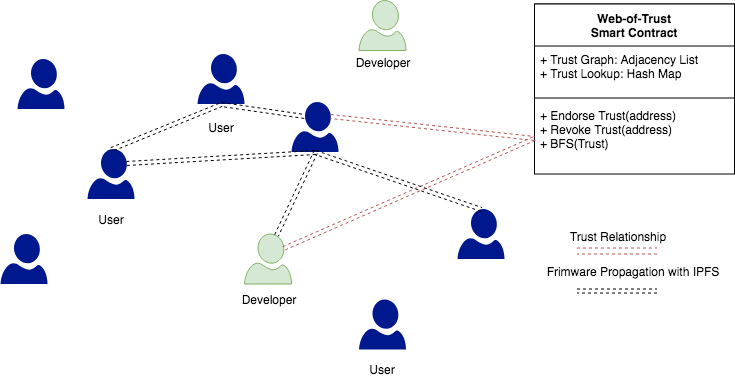
\includegraphics[width=0.95\textwidth]{./pics/IPFS-Archi.png}
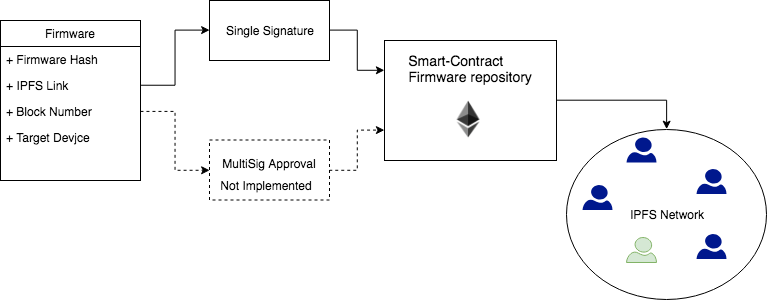
\includegraphics[width=0.95\textwidth]{./pics/Repo-Archi.png}
\caption{Código network architecture diagram. Users are arranged on a graph based on their trust relationship, which is formalized in the Web-of-Trust smart-contract. Firmware metadata are stored on the firmware repository smart-contract and updated using the Código clients. Firmware distribution is on the IPFS layer in which the Código client is uploading/downloading the firmware from the IPFS network.}
\label{fig:arch}
\end{figure}


The first layer of the system lays on top of the Ethereum blockchain. Two smart contracts were developed on top of Ethereum using Solidity \cite{solidity}. At the time of writing Solidity is the only robust language for developing Ethereum Smart Contracts. Solidity is a Javascript type of language that compiles down to Ethereum Virtual Machine instructions that can be executed by the miners. It should be noted that a new language for Ethereum smart contracts, Vyper \cite{vyper}, is also in late alpha stage. The two contracts are independently deployed and communicate with each other using Ethereum transactions. The first contract is responsible for modeling trust while the second is the firmware repository. 

\subsection{Web-of-Trust Smart-Contract}{
The Web-of-Trust smart contract is an implementation of the Web-of-Trust idea in Solidity. The Web-of-Trust is represented as a directed graph and it is implemented using an adjacency list data structure. Nodes can use the web of trust contract independently to allocate their trust to other developers. Figure \ref{fig:webT} illustrates an instance of Web-of-Trust. In this example, Alice trusts Bob with a level 2 trust. Contrary, Bob trusts Alice with a level 1 trust. It is possible and quite likely that the trust graph is not fully connected. For example, in the Web-of-Trust instance in Figure \ref{fig:webT} there is no path from Chloe to Bob. In that case we define Chloe's trust to Alice to be -1. Users are expected to bootstrap their trust profile with the address of other developers that they find from other sources, such as the developers website or GitHub profiles. Then they use the client to allocate their trust towards them. IoT gateways that use the client can bootstrap their trust profile with the address of the manufacturer.

\begin{figure}[!htb]
\centering
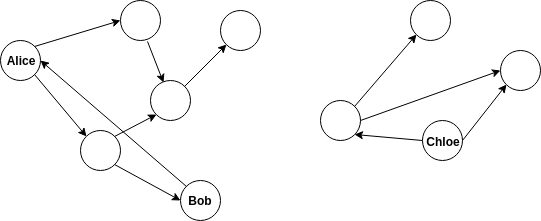
\includegraphics[width=\textwidth]{web_of_trust.png}
\caption{An instance of Web-of-Trust implemented as a directed graph. Trust of party A (vertex) towards B (vertex) is defined as the minimum number of hops (edges) required to reach from A to B. In case no path from A to B exists, we define the trust of A towards B to be -1. }
\label{fig:webT}
\end{figure}

Trust can be allocated to a developer using the endorse trust function of the smart contract. The endorse trust function of the smart contract is performing some logical tests to avoid storing duplicate addresses and appends the new address to the trust graph. As a result, the computational cost of the function and hence the gas cost is independent of the number of trusted users. This is also illustrated in Figure \ref{fig:addTrustGas} that visualizes the gas cost entailed in trusting a new address. It should be noted that in the Ethereum blockchain it more gas is required to change a value from zero to non-zero than from non-zero to non-zero even, if the absolute value difference is the same. As a result, the first call by the user to the function will be more costly. The users have access to the opposite operation which is deallocating trust. The deallocation function needs to iterate over the connections of the users, delete the requested connection and then rearrange the rest of the connections. Therefore the computational cost of the function is $O(trusted\_users)$  and hence the gas cost of the function is increasing linearly in terms of the trusted users. This is also illustrated in Figure \ref{fig:rmTrustGas} that visualizes the gas cost associated with removing the trust from an address. To put the numbers into perspective, with a gas price of 6 GWei, the first call to the endorse trust function would cost 0.00048 Eth, while revoking the trust would cost 0.00033 Eth for a user with 40 trusted addresses.

\begin{figure}[htb!]
\centering
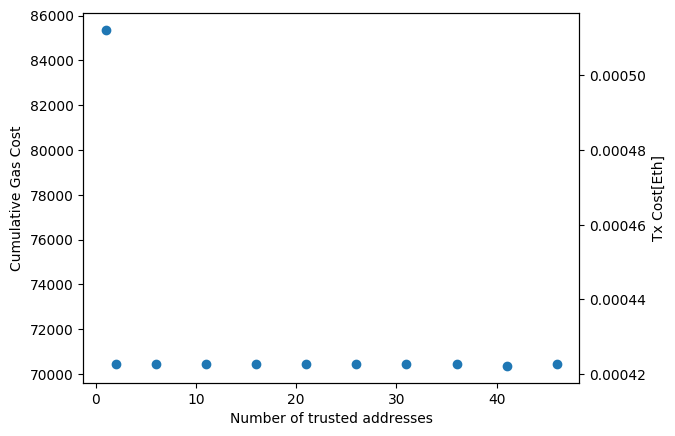
\includegraphics[width=0.95\textwidth]{./pics/endorse_trust.png}
\caption[test]{Gas required and equivalent Eth cost for allocating trust to a user to the Web-of-Trust smart contract.}
\label{fig:addTrustGas}
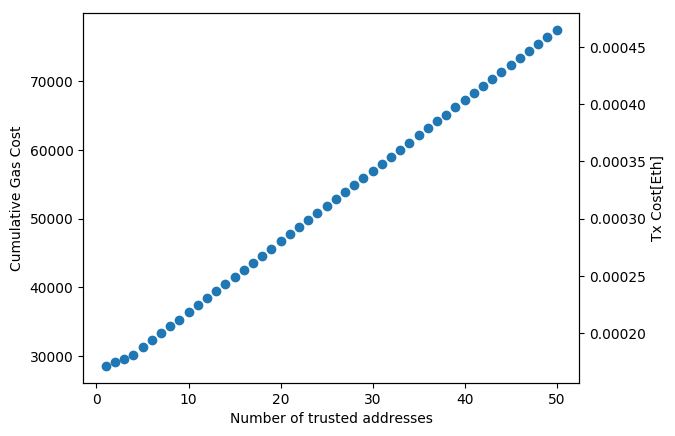
\includegraphics[width=0.95\textwidth]{./pics/revoke_trust.png}
\caption{Gas required and equivalent Eth cost for deallocating trust from a user as a function of the number of trusted addresses to the Web-of-Trust smart contract. Contrary to the trust allocation function, this function transactions costs are linearly correlated with the number of trusted addresses.}
\label{fig:rmTrustGas}
\end{figure}

The last and possibly the most important function of the Web-of-Trust smart contract is the function that calculates the level of trust of user A towards user B. This function does not alter the state of the smart-contract, thus nodes can calculate it locally without the need to perform and consequently pay for a transaction. This function is a classic shortest path graph traversal from origin A to destination B. Theoretically, Djikstra's algorithm \cite{algos} would be the best choice for calculating the shortest path from vertex A to vertex B in a graph with positive edge weights. However, the efficient version of  Djikstra's shortest path algorithm relies on a priority queue data structure. This is a big constrain in Solidity. The reason for that is that custom data structures such as a priority queue are not implemented in the standard library of the language. As a result to use such data-structures one would need to implement them from scratch. The main problem is that in order to use the implemented data-structures one would need to perform a transaction. For example, if someone wants to use their own implementation of a priority queue they would need to create a transaction to initialize a new contract that implements it. This happens even if the custom data structure is used only as a local variable and the function as a whole does not alter the state of the smart-contract. This is due to the fact that smart-contracts, although they syntactically resemble classes they are not. There is no such thing as creating a temporary instance of a contract, operating on it and then at the end of the function deleting the contract instance. As graph traversals are unbounded in size if the function is included in a transaction such operation could result in arbitrarily high transactions cost. Additionally, an attacker could perform the following attack to grief an honest user:

\begin{enumerate}
\item Alice trusts user Eve
\item Alice sends a transaction to calculate her trust towards another user
\item Eve sees the transaction in the mempool and sends multiple transactions to endorse dummy addresses with a high gas price. As a result, Eve's transactions are performed before Alice's.
\item As a result Alice would have to pay more money in transaction fees than she expected in order to perform the requested trust calculation.
\end{enumerate}

Due to the aforementioned reasons, we opted to implement a less efficient traversal method that does not need a priority queue data structure. The traversal is implemented in Solidity using the Breath-First-Search (BFS) algorithm \cite{algos}. The BFS implementation correctness was evaluated with a set of unit tests that checked if the implementation could calculate the trust correctly in the case of cycles in the graph, absence of a path between the destination and the origin and in the case of multiple paths between the destination and the origin.
}

\subsection{Firmware Repository Smart Contract}{
The firmware repository can be thought of as a classic torrent website repository, that is hosted on Ethereum instead of a web-server. The main goal of this smart contract is to store the metadata required to download a firmware. This is a high level requirement that can be translated to a smart-contract, by which developers should be able to upload firmware and users should be able to find all the information they need to download a firmware. In the rest of this section the design of each function of the firmware repository will be discussed. 

Firstly, before going into the details of the smart-contract functions, we must define an appropriate data structure to represent firmware. In Código Network a firmware is represented as struct with the following variables:
\begin{itemize}
  \item  Firmware hash stored as 32-byte array
  \item  IPFS link stored as a string
  \item  Firmware description stored as a string
  \item  Block number stored as 256 bit unsigned integer
  \item  Target device stored as a string
\end{itemize}

The firmware representations follows the guidelines of Code Signing proposed by Cisco \cite{fleischman2002code}. One will observe that there are no signatures of the hash, to validate the author of the firmware. The reason for that is that the signature of the developer is already required by the Ethereum blockchain when he/she uploads the firmware to perform the transaction. Thus it was decided not to store this information in the smart-contract as it already exists in the blockchain. Additionally, the block number is also stored as an indication of the age of the firmware. Assuming that Ethereum maintains the policy of producing blocks at an almost fixed interval, using the block number anyone can calculate at what day the firmware was added to the blockchain.

An improvement that could be made to the current design, which was not implemented during the scope of the project is the introduction of $m-n$ multi-signatures. A group of developers working on the same code-base can publish a smart contract that implements m-n signatures. This behavior is supported by Código Network. Users will merely trust a smart-contract instead of a user address in Web-of-Trust.

In order to upload a firmware to the blockchain, developers need to provide the hash of the firmware, the IPFS link of the firmware, the firmware description and the target device and a PoW nonce. As it was already mentioned, developers need to provide a valid PoW solution in order to upload a new firmware. In general the aim of the PoW system is to allow developers to upload 1-2 firmware updates per day. For each developer, an unsigned integer called challenge, the time of the last submission and the current difficulty are stored. The goal of the developer is to submit a nonce to the smart-contract with the following property:
\begin{align*}
SHA-3(nonce,challenge) \leq difficulty
\end{align*}

The initial PoW difficulty is $10^{77}$ and is divided by $50$ each time a developer pushes a new firmware to the repository within the same day. As the difficulty decreases, the required number of computations increases. If the last proof was submitted more than one day ago, then the difficulty is reseted to its initial value. The challenge is a cryptographic salt that is generated using the following formula:
\begin{align*}
SHA-3(nonce_{prv},challenge_{prv},blockhash)
\end{align*}

Under the assumption that the output of the SHA-3 is uniformly distributed in the range $[0,2^{256}]$, then the probability of generating a valid PoW, $Pr_n[valid|nonce]$, as a function of the number of firmware added, $n$, can be calculated as follows:

\begin{align*}
&initial\_difficulty = 10^{77} \\
&Pr_n[valid|nonce] = \frac{initial\_difficulty}{50^n 2^{256}}
\end{align*}

The $initial\_difficulty$ value was set such that the $Pr_1[valid|nonce] = 0.9$

Furthermore, we can define a set of random variables $Attempts = \{Attempts_n\}$. Each random variable, $Attempts_n$, denotes the number of SHA-3 computations required to calculate a valid PoW if one has added $n$ firmware that day. Each calculation of SHA-3 calculation is a biased Bernoulli trial with probability $p=Pr_k[valid|nonce]$. As a result, $Attempts_n$ is a Geometric distribution \cite{ProbBook}. For each $Attempts_n$ we can calculate the expectated value and variance of the distribution as follows:

\begin{align*}
&\mathbb{E}[Attempts_n] = \frac{1}{Pr_n[valid|nonce]},
&var[Attempts_n] = \frac{1-Pr_n[valid|nonce]}{Pr_n[valid|nonce]^2}
\end{align*}

Based on the formulas above we calculate and present in Table \ref{tab:pow_prob} the expected value and the standard deviation of $Attempts_n$ for $n \in [1,3]$

\begin {table}[htb!]
\caption {The expected number of SHA-3 computations and its standard deviation required to upload multiple firmware within the same day.} \label{tab:pow_prob} 
\begin{center}
 \begin{tabular}{|c| c|c|}
 \hline
 Number of Firmware Added & Average & Std \\ [0.5ex] 
 \hline
  1 & 1.158 & 0.427  \\
  \hline
  2 & 57.896 & 57.394 \\
  \hline
  3 & 2894.802 & 2894.302 \\
  \hline
\end{tabular}
\end{center}
\end {table}

Figure \ref{fig:powCost} graphically illustrates the required SHA-3 computations to upload multiple firmware within the same day under a typical execution. The required SHA-3 computations increase in an exponential rate. Note that the SHA-3 calculations are performed in the client and as a result, the PoW does not increase the transaction costs to add a new firmware by a significant amount.

\begin{figure}[htb!]
\centering
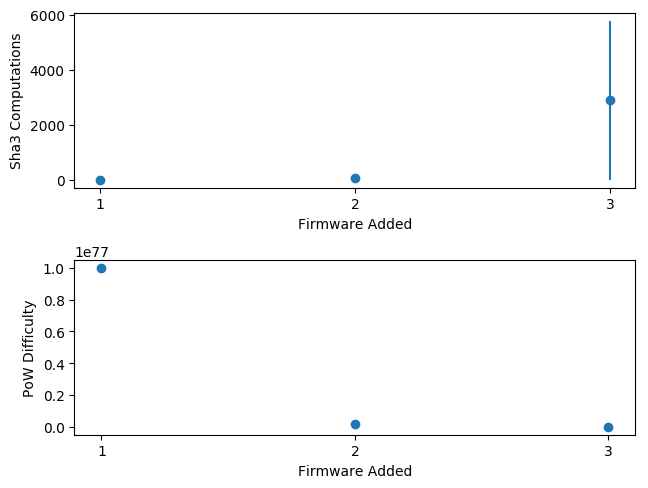
\includegraphics[width=0.95\textwidth]{./pics/pow_cost.png}
\caption{SHA-3 computations required and PoW difficulty as a function of consecutive firmware updates per day. The computation cost increases with an exponential rate as a function of the firmware added}
\label{fig:powCost}
\end{figure}

Each developer is allowed to upload two different versions of the same firmware in the repository, one latest commit version of the firmware and one long-term-support (LTS) version per device type. Although, the number of allowed firmware per developer is two, there is no way to enforce that the latest-lts convention will be followed by the developers. Additionally, developers can use the smart-contract to upload new firmware or edit the description of an existing firmware. Users can query the firmware repository to find a specific firmware, find the firmware from the most trusted developer and find a list of firmware from the most trusted developers. Figure \ref{fig:addGasC} illustrates the transaction costs for adding a new firmware to the repository. The cost is 0.0027 Eth for the first time and the price drops to 0.0009 Eth onwards. In addition to that, there is the extra cost (in terms of CPU cycles and consequently electricity) for finding the appropriate nonce and solve the PoW.

\begin{figure}[htb!]
\centering
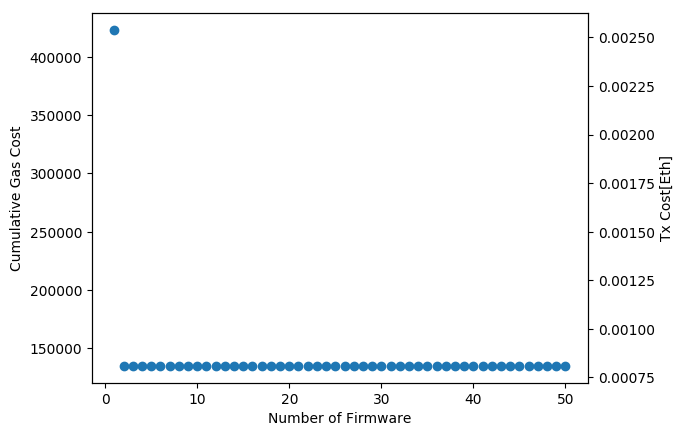
\includegraphics[width=0.91\textwidth]{./pics/add_firmware.png}
\caption{Gas required and equivalent Eth cost for uploading a new firmware to the firmware repository smart-contract}
\label{fig:addGasC}
\end{figure}

}

Users can view and then download the most trusted firmware, or retrieve a list of trusted firmware. These functions merely browse through the smart-contract data without modifying its state. As a result, these functions can be computed without a transaction. This comes with an additional privacy advantage. As users, do not have to make a transaction to download a firmware, then no personal information about the type of devices they own is leaked in the blockchain.

\subsection{Código Network Clients}{
To interact with the blockchain layer and download/upload a firmware from/to the IPFS network, a user and developer client were developed. These clients were designed to make the process of uploading and downloading new firmware smoother in an user friendly way. As a decentralized system, Código network was designed in a away that does not rely on the developed clients to work. The reason for that was to avoid making the clients an implicit centralization point. As a result, the developed smart-contracts are fully autonomous and the user can interact with them with their favorite blockchain enabled tool, without installing the Código client. The same applies to the IPFS layer. Users can use the command-line-interface of the IPFS client directly to download the firmware without relying on the firmware.

To maximize the usability of the client, the option of using remote IPFS and Ethereum nodes is offered. This is particularly useful for IoT devices that do not have the luxury of running a full Ethereum and IPFS node locally. Ideally the user can run an Ethereum and an IPFS node on her computer and then contact those from the IoT devices to perform the calculations. Furthermore, both clients are software applications that rely on the existence of clients that will make the transactions. This means that the clients do not store the private keys of the users nor make transactions themselves. The user would need to connect the client with their Ethereum wallet to perform transactions. This is a responsibility that burdens the user. Finally, both clients were developed using the Python bindings of the Qt framework \cite{summerfield2007rapid}.

The developers client can be used to upload a new firmware directly to the blockchain and to the IPFS. The main benefit of using the developer is that firmware are uploaded to both  Ethereum and IPFS in a congruent way. Figure \ref{fig:devClient} illustrates the developer client UI. The user client is responsible for querying the blockchain to find firmware updates and then download the latest firmware. The user-client also implements the functions of the smart-contracts that do not require transactions. This gives the flexibility to the user to choose between running the smart-contract functions locally on the Ethereum Virtual Machine or making the calculations locally using the client. Figure \ref{fig:userClient} illustrates the user client UI.

\begin{figure}[h!]
\centering
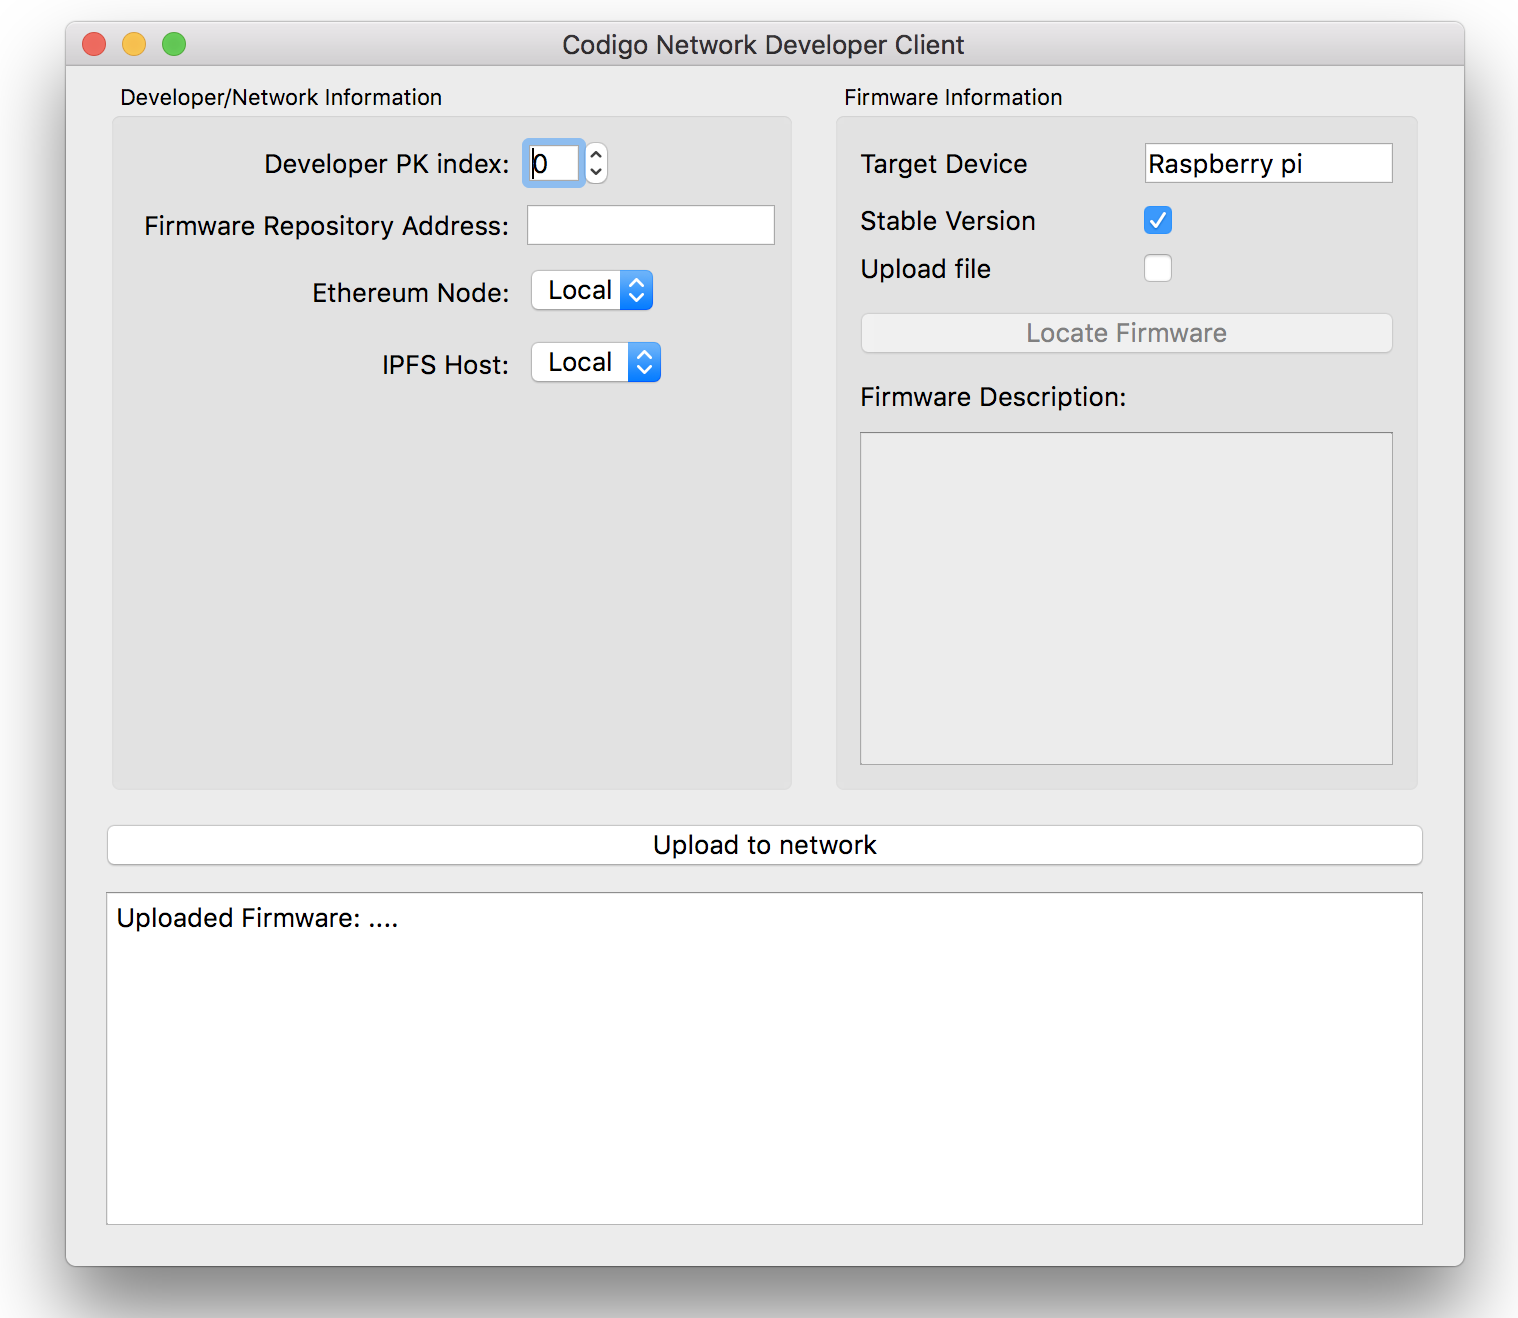
\includegraphics[width=0.95\textwidth]{./pics/Developer_client.png}
\caption{Código Network developer client}
\label{fig:devClient}
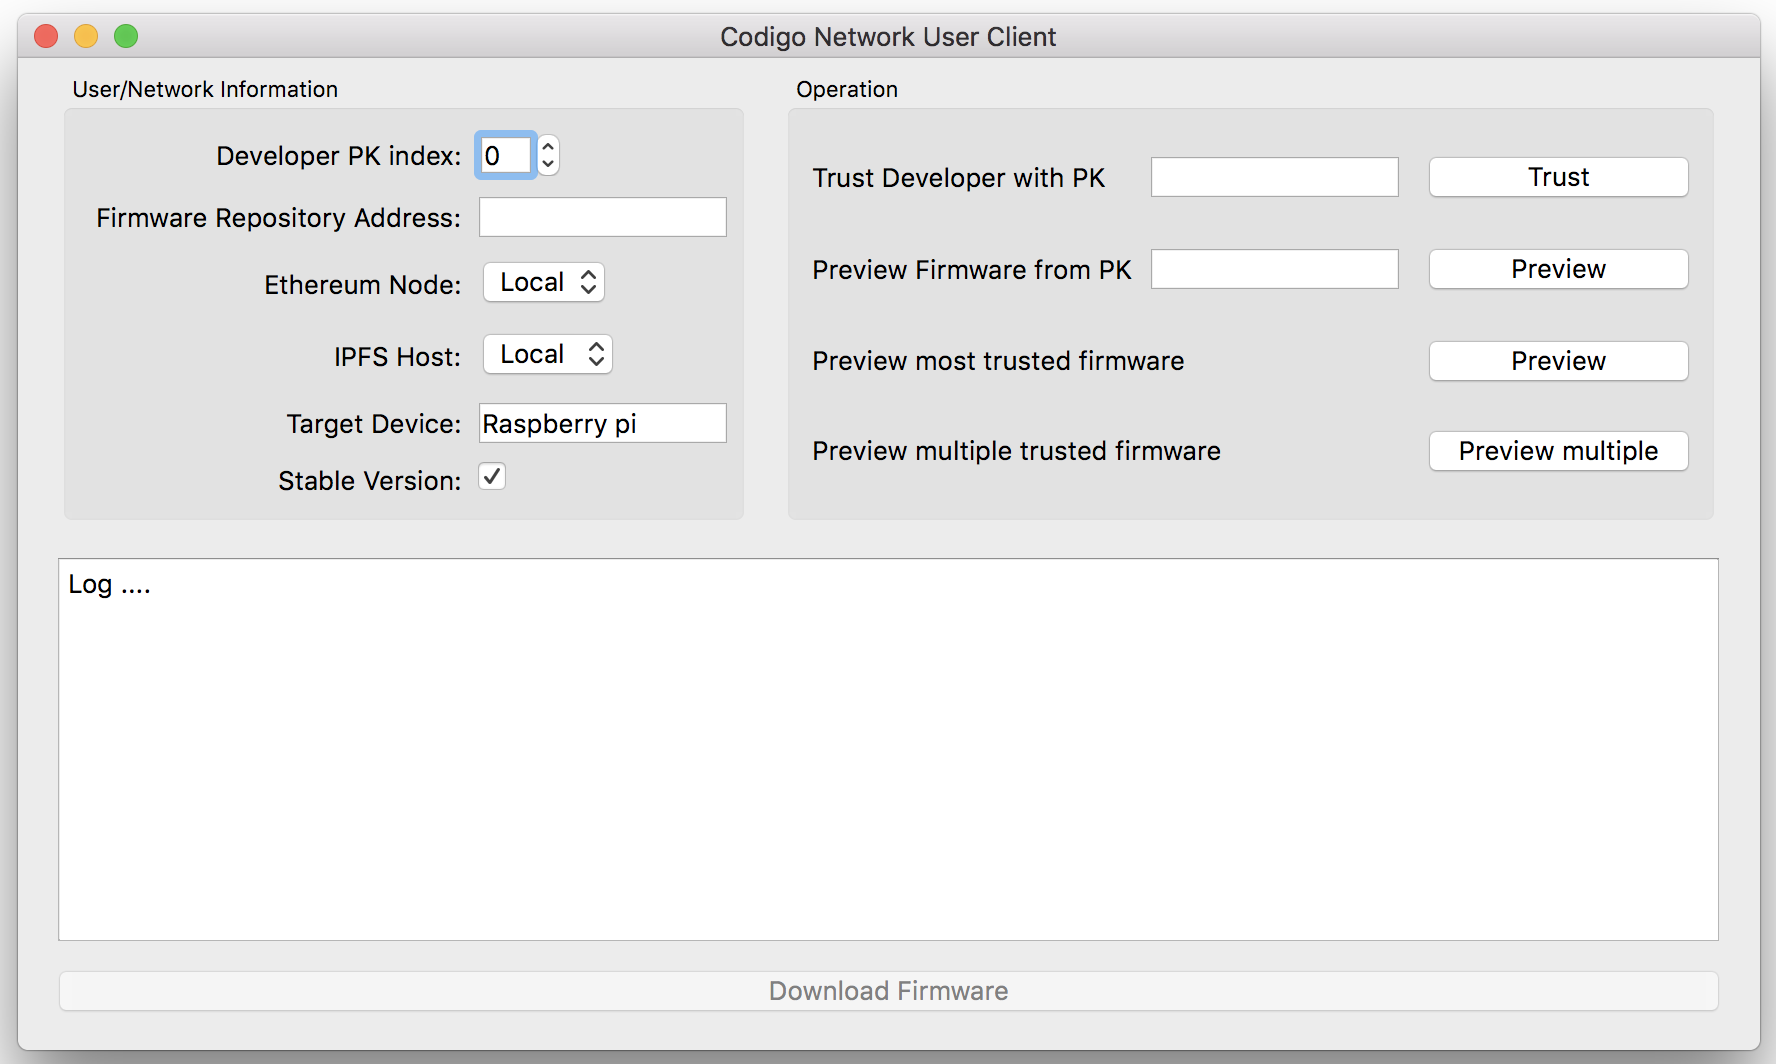
\includegraphics[width=0.95\textwidth]{./pics/user-client.png}
\caption{Código Network user client}
\label{fig:userClient}
\end{figure}
}
}
}

\chapter{Código Network Evaluation}\label{chap:CNeval}{

Until this point the report motivated and descrobed the design of Código network, and evaluated the performance of the developed smart-contracts. As with any other distributed system, it is critical to measure Código network performance and evaluate how it stands against other competing technologies. Therefore, in this section the attention is shifted towards evaluating the efficiency of the developed framework in distributing a file from the developer to the rest of the users. The performance of the system is evaluated experimentally and is compared against the Client-Server model and the BitTorrent protocol. The comparison is based on the concept of average delay. Average delay is a measure that expresses the average time required for $k$ users to simultaneously download the same firmware. Additionally we explore the issue of redundancy and overheads in firmware distribution.

\section{Performance Experiments}{
\subsection{Experiment Setting}{

To evaluate the performance of the network we consider the following experiment setting. A single user creates a new firmware and $k$ users simultaneously download it. The firmware size is 10MB.  For this set of experiments all nodes are in the same Local Area Network and have 0\% packet loss and minimal latency. In particular, since all the communications are within the localhost, we have only the latency associated with the system processing the request. All the experiments are executed in the Google Cloud Compute engine using a virtual machine with 64 CPUs and 240 GB memory, and Ubuntu 16.04 LTS as the operating system.

Our generic simulation algorithm is shown in Algorithm \ref{alg:simulation}. There the functions $upload\_file()$ and $download\_file()$  depend on the framework. For example, for the Client-Server model, the $upload\_file()$ would be starting the file distribution server and $download\_file()$ would be making an HTTP request to that server. Furthermore, the $download()$ function in the simulation is used in asynchronous manner to capture the idea of multiple nodes downloading the same file at the same time. In the $download()$ function we additionally may use mutexes to avoid data racing condition, if the append function is not thread safe in the language used to implement the logic of the simulation. For example in Python (used for Client-Server simulation) append is thread safe whereas in Golang (used for IPFS simulation) we use the Golang channels. Algorithm \ref{alg:simulation} is used by Algorithm \ref{alg:simulationFull} to execute the simulation for $k$ users where $k \in [1,120]$ 

\begin{algorithm}
\caption{Core Simulation}\label{alg:simulation}
\begin{algorithmic}[1]

\Function{Simulation\_Core}{users}
    \State {$upload\_file()$}
    \State $delay[]$
    \Function{download}{}
        \State {$start$ $\gets$ {$now$}}
        \State {$download\_file()$}
        \State {$end$ $\gets$ {$now$}}
        \State {$delay[]$ $\gets$ $delay[]$ + {$(end - start)$}}
    \EndFunction
    
    \For{$user \gets 1$ to $users$}                    
        \State \text{async} $DOWNLOAD()$
    \EndFor
    \State \text{Wait for all calls to finish}
    \State {$calculate\_statistics(delay)$}
    \EndFunction
    \end{algorithmic}
\end{algorithm}

\begin{algorithm}
\caption{Simulation Procedure}\label{alg:simulationFull}
\begin{algorithmic}[1]

    \For{$k \gets 1$ to $max\_users$}                    
        \State $Simulation\_Core(k)$
    \EndFor
\end{algorithmic}
\end{algorithm}

In the $calculate\_statistics(delay)$, we calculate the \textit{average delay} ($\bar{d}$) in retrieving the file as follows:

\begin{align*}
\bar{d} = \frac{\sum_{i=1}^{k}{t_i}}{k}
\end{align*}

where 

\begin{itemize}
\item $t_i$ is the time that it took user $i$ to download the file.
\item $k$ is the number of users that simultaneously retrieve the file.
\end{itemize}

Similarly, we calculate and use other useful metrics such as the standard deviation of the delay, the minimum and the maximum. 

To implement the simulations the following tools were utilized:
\begin{enumerate}
\item \textbf{The IPTB framework} \footnote{Forked IPTB: \url{https://github.com/davinci26/iptb}}: The official IPTB framework was forked and expanded to meet our simulation requirements. The simulation flow and the calculations above were implemented in IPTB. The IPTB framework spawns multiple IPFS nodes in a single machine and each node is unaware of the existence of the rest of the local nodes. When the simulation starts, nodes asynchronously start downloading the file. The results are combined together when all nodes download the file. Our simulation framework is currently under code review and will be integrated in the official IPTB framework to measure the performance of IPFS \footnote{Pull request: \url{https://github.com/ipfs/iptb/pull/65}}.
\item \textbf{BitTorrent simulation tool \footnote{BitTorrent Simulator: \url{https://github.com/thejosh223/cs198mojo/tree/master/PeerSimCode/Peersim-BitTorrent}}}: This tool utilizes the P2P simulation library \cite{p2p09-peersim}. The simulation tool is a lightweight implementation of the BitTorrent protocol that does not actually transfer the file but simulates the transfer as a set of messages. Note that the BitTorrent simulation is based on fixed time intervals set to 1 second, as a result all the results produced by the simulation have an error margin of $\pm$ 0.49 seconds
\item \textbf{Client-Server Simulator}: This consists of a pair of Python programs responsible for implementing a Server and a set of $k$ clients. The tailor made Python flask server \cite{flask} responds to HTTP requests with a 10MB file. The set of $k$ clients  are implemented as different threads. The client program spawns $k$ threads that request the file simultaneously from the server.
\end{enumerate}
}
An important detail for the P2P systems, namely IPFS and BitTorrent, is that users close their IPFS and BitTorrent clients when all the other users in the system have finished downloading the firmware. This is a strong assumption that works in favor of performance for the decentralized systems, as the users who download the file early do not abort the protocol but remain as file seeders. 

\subsection{Results}{

In terms of performance the client-server is able to outperform both decentralized systems in file distribution. This is illustrated in Figure \ref{fig:CSPerf} that shows that distributing a single file to 100 users takes ~2.491 seconds. The main issue with this approach is that by definition the cloud server is single point of failure in the system. As a result, the distribution of the firmware is limited to the ability of the manufacturer to afford Cloud computing resources. To put things into perspective the cost of the instance used to perform the simulations is \$ 20,717.04 per year according to the Google Cloud Billing plan. Additionally, as the cost of vertical scaling in web applications increases exponentially, sustaining even higher number of users would result in exponentially higher costs.

\begin{figure}[!htb]
\centering
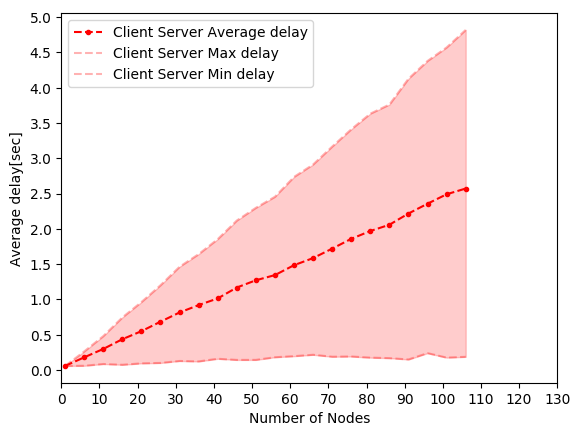
\includegraphics[width=\textwidth]{./results/client-server.png}
\caption{Average delay in downloading a single 10MByte file from a Python Flask server, as a function of the number of users, that want to download the file. Each data point refers to a single execution of Algorithm \ref{alg:simulation}.}
\label{fig:CSPerf}
\end{figure}

IPFS network which constitutes the framework that Código network uses to distribute firmware to the users has a solid performance that deteriorates as the numbers of users increases. The first observation that should be made is that the average time required to download the same file, when 100 nodes want the file, using IPFS is 22.9 times slower than the client-server model. The more worrying part is not that IPFS is orders of magnitude slower than client-server, but that the average delay is increasing almost linearly as the number of nodes increases. Intuitively we expect that, in a P2P system as the number of nodes increase, both the number of seeders and the number of leechers increase and the load is balanced among the users. This should guarantee a better performance at scale. Figure \ref{fig:IPFSPerf} illustrates the performance of IPFS network as the number of users requesting the file increases.

\begin{figure}[!htb]
\centering
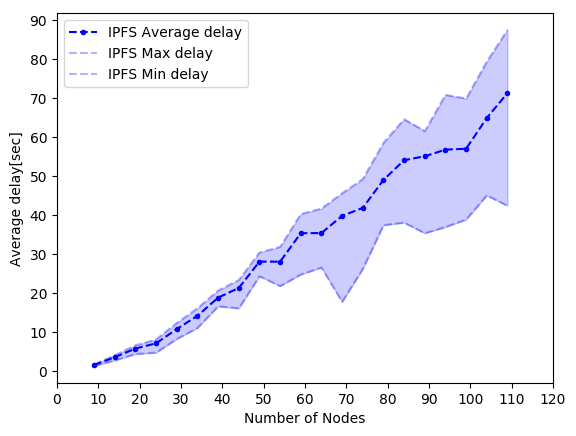
\includegraphics[width=\textwidth]{./results/ipfs-perf.png}
\caption{Average delay in downloading a single 10MByte file using the IPFS network. Even though it is a P2P network it seems that the average time required to download the file increases as the number of users increases. Each data point refers to a single execution of Algorithm \ref{alg:simulation}}
\label{fig:IPFSPerf}
\end{figure}

To understand why our intuition was incorrect, we decided to delve deeper into the implementation of the IPFS Bitswap protocol that is responsible for the file distribution. We discovered that the current design of block swapping has a flaw that causes the performance deterioration. In particular what is happening now is that nodes that want to download a file share to the network a \textit{wantlist} of the blocks they need. Remember, each file in IPFS is split in a set of blocks. Then other seeders, see the \textit{wantlist} of other users and send them the block. For example, if Alice wants to download a file that consists of four blocks (b1,b2,b3,b4) she will publish a wantlist that consists of $[b1,b2,b3,b4]$. Then users Bob and Charlie who already have the blocks and want to participate in the exchange will start sending Alice raw data.

At the time of receiving data from Bob and Charlie, Alice does not know which block she receives. As a result, she will wait until the transmission is over and then calculate the hash of the received bytes. If the hash matches one of the blocks in the wantlist she removes it from her wantlist. The problem is that Alice does not know which block she receives before the transmission is over. Additionally, Bob does not know that Charlie is also sending a block to Alice and vice versa. As a result as the number of users increase, Alice would spend her bandwith in publishing her wantlist to multiple nodes and receiving duplicate blocks from other nodes. This result is shown in Figure \ref{fig:IPFSDups} which illustrates the total number of duplicate blocks transmitted in the network in terms of the nodes participating in the exchange of a single file. It can be observed that there is a linear increase in the number of duplicate blocks as the number of users in the swarm increase. This lack of coordination between block senders and receivers is the reason behind the performance deterioration of IPFS as the number of users interested in a single file increase.

\begin{figure}[!htb]
\centering
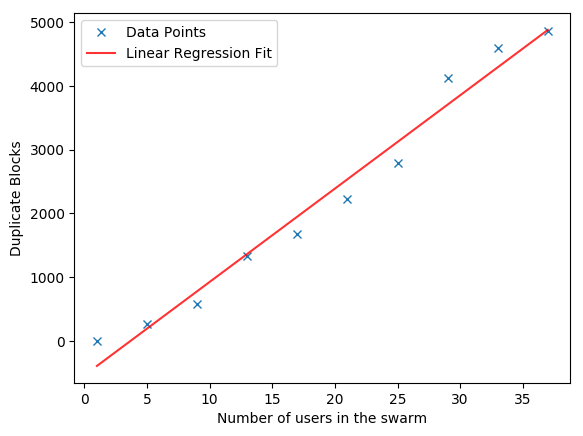
\includegraphics[width=\textwidth]{./results/ipfs_duplicates.png}
\caption{Number of duplicate blocks exchanged in the IPFS newtwork as a function of number of users in the swarm. It can observed that as the number of nodes interested in a single file increases then more duplicate blocks are transmitted. Due to the lack of communication between network users, nodes end up wasting resources to exchange duplicate blocks.}
\label{fig:IPFSDups}
\end{figure}

The content distribution is a crucial component of Código network. The fact that IPFS performance is way worse than the Client-Server model is not a major concern for Código network. One of the motivations for designing a decentralized firmware distribution network was to enable a robust model for open-source development of firmware. This is not possible under the Client-Server model, as the operator of the server is an implicit trusted party and a single point of failure. Additionally, another advantage of IPFS against Client-Server model is that it does not require an Internet connection to work. In a network of multiple IoT devices connected via WLAN, if one of the devices has the file then it can distribute it via WLAN to the rest. Furthermore, we simulated a situation where all devices are in the WLAN and share the firmware. However, consider the case in which the distribution server is the US and the nodes requesting the file are in Europe. IPFS would prioritize devices with better connection and thus have a better performance under those conditions. This comes from the fact that IPFS uses the "tit-for-tat" mechanism. For example, let Alice be in the EU, Bob in the USA and Charlie also in EU. Then Alice would have better connection speed with Charlie (EU) compared to Bob (USA). As a result, due to the incentives of the protocol, Alice would engage in more block transactions with Charlie because he is uploading more data at a fixed time interval.

The last question that we chose to address in this project is how IPFS compares against BitTorrent in terms of performance. As both systems are decentralized this comparison will be more meaningful. It can be observed that BitTorrent is on average slower than IPFS and by a big margin. Additionally, the BitTorrent protocol (different BitTorrent clients can optimize around this problem) is not fair towards the users, as the difference between the minimum and the maximum download time could be different by orders of magnitutde. Figure \ref{fig:BitTorrentPerf} demonstrates the performance of BitTorrent protocol in distributing a single file to multiple nodes as the numbers of nodes increases. However, as the number of nodes increases, give the performance of IPFS we assume that there exists a sufficiently large number of nodes for with BitTorrent will outperform IPFS.

\begin{figure}[!htb]
\centering
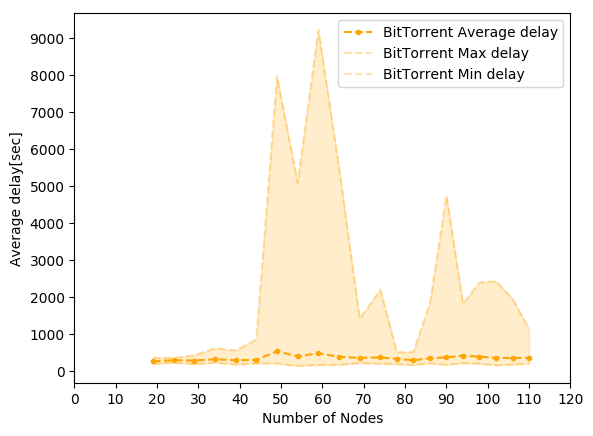
\includegraphics[width=\textwidth]{./results/BitTorrent.png}
\caption{Average delay in downloading a single 10MByte file using the BitTorrent network. The BitTorrent protocol seems not to be affected on average by the number of users in the swarm.}
\label{fig:BitTorrentPerf}
\end{figure}

The aforementioned comparison between content distribution frameworks is summarized in Table \ref{tab:all_comp} in which the average, std, median, min, max delay are presented for100 users trying to simultaneously download a single 10 MByte file.

\begin {table}[htb!]
\caption {Comparison between Client-Server model, BitTorrent and IPFS in the distribution of a single file to 100 users} \label{tab:all_comp} 
\begin{center}
 \begin{tabular}{|c| c|c |c | c| c |}
 \hline
  & \multicolumn{5}{|c|}{Delay[sec]} \\
 \hline
 Model & Average& Std & Median & Min & Max \\ [0.5ex] 
 \hline
  Client-Server & 2.491 & 1.259 & 2.549 & 0.176 & 4.571 \\
  \hline
  BitTorrent & 331.489 & 82.552 & 330.0 $\pm$ 0.49 & 180.0 $\pm$ 0.49 & 590.0 $\pm$ 0.49 \\
  \hline
  IPFS & 57.053 & 5.958 & 57.938 & 38.910 & 69.931 \\
  \hline
\end{tabular}
\end{center}
\end {table}

}
}
}

\chapter{Conclusion and Future Work} \label{chap:conc}{
\section{Project Analysis}{

To conclude the project, we will analyze holistically the design in terms of the requirements that were set in Section \ref{sec:PD}. Overall the goal of the project which was to develop a decentralized firmware distribution network was achieved. Specifically, we can examine each goal individually:
\begin{itemize}
    \item \textbf{No single point of failure}: This requirement is easily satisfied from the Ethereum blockchain and the IPFS network. In our framework device manufacturers are the initial trusted developer of the device. However, this does not prohibit other developers from developing firmware for a given device. As a result, Código network not only enables open source firmware development but also provides an infrastructure that also promotes it.
    \item \textbf{Equivalent security with code signing}: Essentially the code signing procedure is followed but in, different way. The hash of the firmware and the signature of the hash are submitted to the Ethereum network when the firmware is uploaded. When users download a file from the IPFS network they, already have a signed hash and consequently they can compare the hash of the file with the hash of the file available in the smart-contract. In the code signing procedure, the developer also includes a certificate from a certificate authority that authenticates her public key. In Código network, instead of relying on certificate authorities for trusted developers, we deployed the Web-of-Trust infrastructure.
    \item \textbf{Transparency}: Every uploaded firmware is associated with a specific public key, linking to a developer. Furthermore, due to the Web-of-Trust, developers can not change their public key and expect to have their firmware viewed by a lot of users. As uploading a firmware requires an Ethereum transaction every firmware update is visible by parsing the Ethereum blockchain. Finally, as long as Ethereum is secure, developers are not able to edit or delete a firmware update from the blockchain.
    \item \textbf{Scalability}: As seen from the results IPFS is able to outperform the vanilla implementation of the BitTorrent protocol. IPFS is still slower than the client-server model. However, given the funding that Protocol Labs received and the fact that the IPFS community is already working on alleviating the duplicate-blocks issue, we are positive that the performance of IPFS would improve dramatically in the forseable future.
\end{itemize}

}
\section{Ethical Considerations}{

In the design of the Código network firmware repository smart-contract, we say that "The firmware repository can be thought of as a classic torrent website repository". The question that remains is what stops users from using this as an illegal file distribution framework. Nothing in the code can stop users from uploading illegal movies in the Código network firmware repository smart-contract and using the IPFS link to distribute those movies. On the other hand, users that only want to download a firmware are not affected by this as they have a way to curate the downloaded files and trust developers they know or that the manufacturer trusts. On the other hand, nothing stops an illegal content distribution community from forming their own strongly connected component in the trust graph and use the framework to distribute illegal content.

Sadly, the most pragmatic answer to this ethical consideration is that it is unavoidable. Código network is firmware distribution network, or even better a fully decentralized file distribution network. As any other new technology, Código network is a double-edged sword. Especially considering that in a decentralized system there is no central authority, that can curate and ban illegal behaviors.  The author truly believes that any fully decentralized system is a true reflection of the society. Agents engaging in illegal activities are a part of our society but the majority of agents are willing to participate in society according to its rules. Additionally, it should be noted that transactions in Código network and file uploads are not anonymous. As a result, users that deviate from the core concept of decentralized firmware distribution should understand that they are doing it in a public and transparent way.


}
\section{Proposal for Future Work}{

Although Código network managed to satisfy the goals set on Section \ref{sec:PD}, it could be further improved. The areas of improvement could be:

\begin{itemize}
    \item \textbf{Multi-signatures}: incorporate $m-n$ multi-signatures during the signing process of the firmware. Multi-signature accounts can be implemented in the form of Ethereum smart-contracts. Users would then have to trust the smart-contract providing the multi-signature instead of trusting individual developers.
    \item \textbf{Content curation}: The basis for this idea would be nodes to execute the firmware in a sandbox environment, based on secure hardware. Then classify the firmware as malicious or honest and construct a cryptographic proof of proper execution of the experiment. This proof could be submitted on the firmware repository smart contract in order to delete a firmware.
    \item \textbf{Mechanism design}: In the current design, developers are required to pay fees in order to submit a firmware to the repository. Additionally, honest developers that provide value to the community obtain no implicit or explicit reward. In Github, for example, developers are implicitly rewarded with repository stars or community recognition for their work. Código network could introduce a utility token via an ICO and reward developers that offer value to the community. However, the introduction of such a coin is not a trivial task, due to  the decentralized nature of the system.
\end{itemize}


}
}
%% ... etc ...

%%%%%%%%
%% Any appendices should go here. The appendix files should look just like the
%% chapter files.
%\appendix
%\chapter{Aliquam erat volutpat}

(If you're wondering what all this weirdness is, check out\\
http://www.subterrane.com/loremipsum.shtml)

Aliquam erat volutpat. Phasellus sed tortor at metus luctus venenatis.
Etiam vel dolor vel lectus elementum adipiscing. Donec sit amet dolor. In
hac habitasse platea dictumst. Nullam bibendum. Etiam eget mauris non velit
faucibus volutpat. Ut ultrices nonummy mi. Praesent convallis, tellus eget
posuere auctor, est est mollis risus, vitae fringilla orci nisl vel erat.
Morbi ultricies. Proin consequat. Praesent consequat nulla a mauris.
Vivamus tellus. 

\section{Proin consequat}

Sed blandit nunc id massa. Integer dictum euismod tellus. Sed metus nunc,
rhoncus ut, volutpat in, lacinia ac, dolor. Vestibulum quis augue
vel dui volutpat eleifend. Praesent vulputate mattis leo. Phasellus pretium
semper libero. Mauris a enim non pede convallis suscipit. Suspendisse nibh
diam, luctus in, cursus at, dignissim nec, pede. Aenean semper massa.
Pellentesque habitant morbi tristique senectus et netus et malesuada fames ac
turpis egestas. Nullam a pede ut ligula viverra vehicula. Sed augue mi,
rhoncus ut, ultrices sed, tincidunt eget, libero. Nam quis dolor. Nunc
fermentum hendrerit arcu. Integer non enim. Aenean blandit velit et felis. Cum
sociis natoque penatibus et magnis dis parturient montes, nascetur ridiculus
mus. Curabitur nonummy malesuada pede. Nunc et enim. Quisque dui. Pellentesque
in felis. 

Sed id mi. Pellentesque pede leo, auctor et, interdum eu, posuere semper,
nisl. Morbi commodo euismod wisi. Cras ornare mauris et erat. Duis neque
neque, pretium ut, bibendum nec, ultrices a, lacus. Nullam lobortis. Ut
luctus, diam non tempus pellentesque, dui justo consequat ligula, eu
consectetuer tortor diam vel dui. 

\begin{figure}
    \begin{center}
        A figure.
        \caption{Nunc lacinia}
    \end{center}
\end{figure}

Phasellus porttitor. In pede lacus, convallis semper, fermentum eu,
vehicula quis, dui. Ut sodales pede sed est. Cras lacinia. Nulla ac augue
in lectus sodales ultricies. Nam velit nunc, convallis ac, ullamcorper
semper, malesuada vel, eros. Nunc risus. Vestibulum ac erat. Sed id justo
id nibh viverra facilisis. Curabitur laoreet. Nunc sodales odio at mauris.
Vestibulum tincidunt sem eget pede. Nulla nec risus non wisi varius porta.
Morbi nibh. Donec lacus. Vestibulum ante ipsum primis in faucibus orci
luctus et ultrices posuere cubilia Curae; Vestibulum lectus. Suspendisse
sed dui. 

Nunc lacinia, sapien nec fermentum pretium, turpis elit egestas metus, a
interdum tellus justo semper neque. Integer quis purus semper metus
vestibulum pharetra. Maecenas commodo fermentum wisi. Pellentesque diam.
Proin sit amet orci. Praesent auctor. Sed tortor. Sed sodales aliquam diam.
Vivamus cursus leo nec velit. Sed non pede. Nulla tempor imperdiet est.
Curabitur ornare cursus ante. Sed varius lobortis quam. Quisque ac arcu id
wisi ultrices pellentesque. Pellentesque eleifend consequat ipsum. Fusce
vestibulum sagittis lectus. Fusce risus. Duis felis. Suspendisse justo.
Integer ut libero a purus egestas luctus. Mauris dictum augue a enim.
Vivamus sodales placerat ipsum. Nunc lacus. 

\begin{quote}
Curabitur dictum. Donec vestibulum diam nec lacus. Nulla convallis, eros
vitae varius volutpat, erat quam facilisis purus, in accumsan dolor felis
vitae nunc. 
\end{quote}

Aliquam erat volutpat. Phasellus sed tortor at metus luctus venenatis.
Etiam vel dolor vel lectus elementum adipiscing. Donec sit amet dolor. In
hac habitasse platea dictumst. Nullam bibendum. Etiam eget mauris non velit
faucibus volutpat. \footnote{Ut ultrices nonummy mi. Praesent convallis, tellus eget
posuere auctor, est est mollis risus, vitae fringilla orci nisl vel erat.
Morbi ultricies.} Proin consequat. Praesent consequat nulla a mauris.
Vivamus tellus. 

Phasellus porttitor. In pede lacus, convallis semper, fermentum eu,
vehicula quis, dui. Ut sodales pede sed est. Cras lacinia. Nulla ac augue
in lectus sodales ultricies. Nam velit nunc, convallis ac, ullamcorper
semper, malesuada vel, eros. Nunc risus. Vestibulum ac erat. Sed id justo
id nibh viverra facilisis. Curabitur laoreet. Nunc sodales odio at mauris.
Vestibulum tincidunt sem eget pede. Nulla nec risus non wisi varius porta.
Morbi nibh. Donec lacus. Vestibulum ante ipsum primis in faucibus orci
luctus et ultrices posuere cubilia Curae; Vestibulum lectus. Suspendisse
sed dui. 

Sed id mi. Pellentesque pede leo, auctor et, interdum eu, posuere semper,
nisl. Morbi commodo euismod wisi. Cras ornare mauris et erat. Duis neque
neque, pretium ut, bibendum nec, ultrices a, lacus. Nullam lobortis. Ut
luctus, diam non tempus pellentesque, dui justo consequat ligula, eu
consectetuer tortor diam vel dui. 


%% ... etc...

%% Choose your favourite bibliography style here.
\bibliographystyle{acm}


%% If you want the bibliography single-spaced (which is allowed), uncomment
%% the next line.
%\singlespace

%% Specify the bibliography file. Default is thesis.bib.
\bibliography{thesis}

%% ... that's all, folks!
\end{document}
